\documentclass[10pt]{beamer}
\usepackage{amsmath}
\usepackage{amssymb}
\usepackage{geometry}
\usepackage{graphicx}
\usepackage{url}
\usepackage{hyperref} 
\usepackage{bm}

\makeatletter
\let \@sverbatim \@verbatim
\def \@verbatim {\@sverbatim \verbatimplus}
{\catcode`'=13 \gdef \verbatimplus{\catcode`'=13 \chardef '=13 }} 
\makeatother

\begin{document}

%-----------------------------------------
\begin{frame}
\large
Lecture 4:\\ 
Diagnostics for Simple Linear Regression\\
STAT 632, Spring 2020
\end{frame}

%-----------------------------------------
\begin{frame}{Anscombe's Four Data Sets}
\begin{figure}
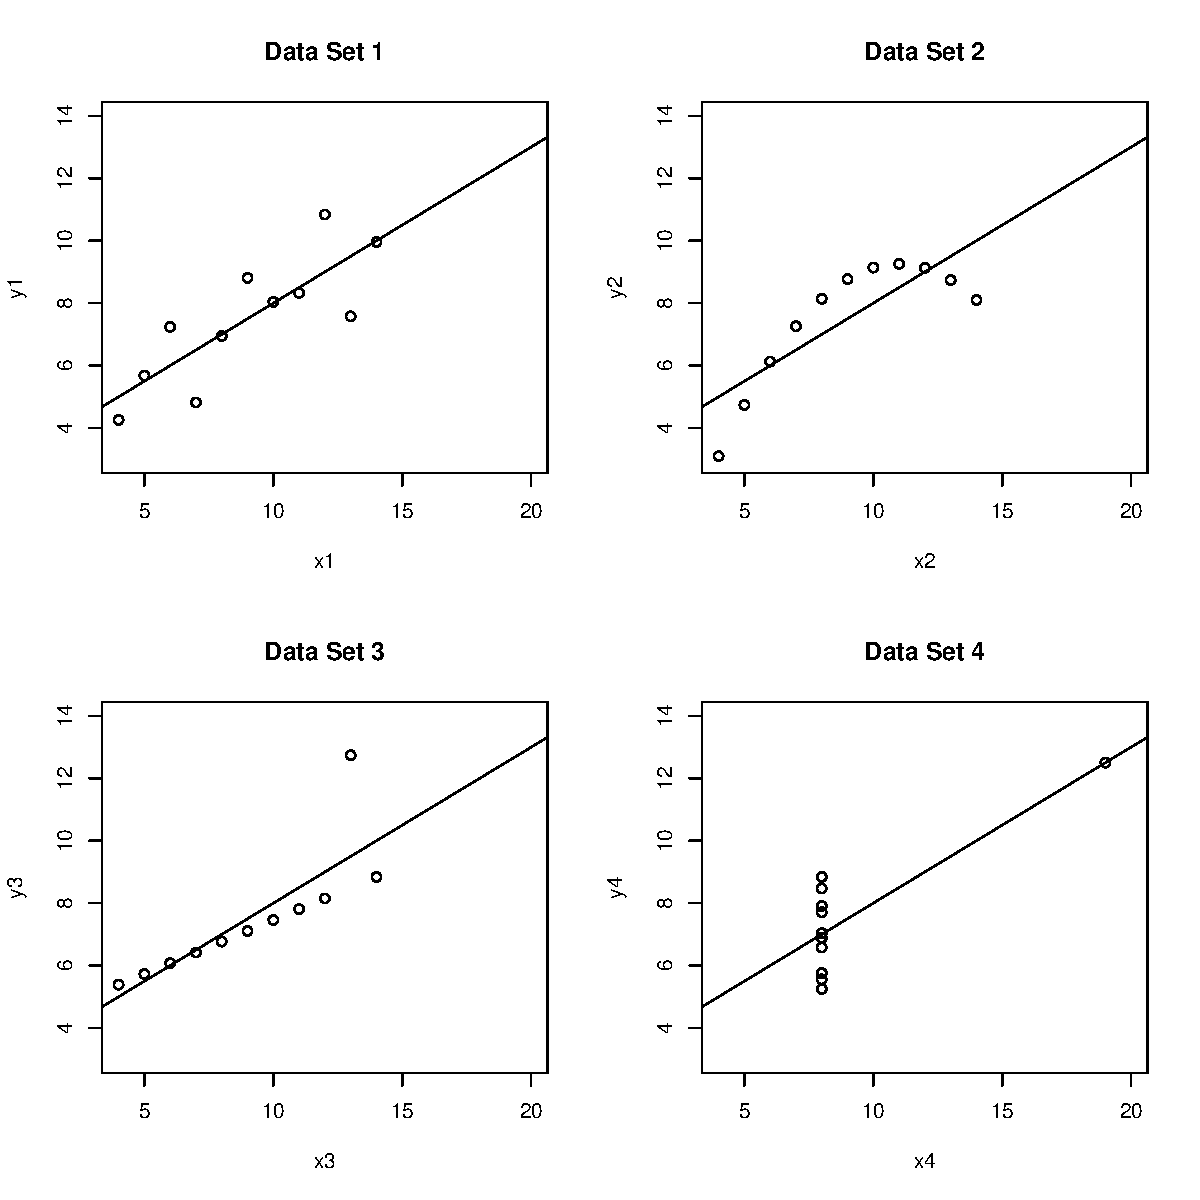
\includegraphics[scale=0.4]{figure/anscombe.pdf}
\end{figure}
\end{frame}

\begin{frame}{Anscombe's Four Data Sets}
\vspace{-3cm}
\begin{itemize}
\item All four data sets have the same least squares regression line, $\hat{y} = 3.0 + 0.5x$, and the same $R^2 = 0.67$.
\vspace{5pt}
\item For which data set(s) is fitting a simple linear regression model reasonable?
%\item A simple linear regression model is only reasonable for the first data set.  The second data set has an obvious curved (quadratic) relationship.  The third data set has an outlier that should be investigated.  For the fourth data set, the slope of the regression line is determined by a single point.
% \vspace{5pt}
% \item This example illustrates the importance of looking at the data first, and assessing whether or not a linear regression model is reasonable. 
% \vspace{5pt}
% \item Regression summaries (e.g., $R^2$) can be misleading without also conducting some exploratory analysis.
\end{itemize}
\end{frame}

%-----------------------------------------
\begin{frame}{Regression Diagnostics}
\begin{itemize}
%\item The linear regression model makes assumptions about linearity between the explanatory and response variable (i.e., $E(Y|X=x) = \beta_0 + \beta_1 x$); and constant variance, independence, and normality in the errors (i.e., $e_i \sim N(0,\sigma^2)$).
\item Assumptions of SLR model 
\begin{enumerate}
\item Linearity:
\vspace{10pt}
\item Independence:
\vspace{10pt}
\item Constant Variance:
\vspace{10pt}
\item Normality:
\end{enumerate}
\vspace{10pt}
\item Regression diagnostics are a set of techniques (both numerical and graphical) that can be used to check the validity of these assumptions.
\vspace{5pt}
\item Regression diagnostics often suggest improvements, which means model building is an iterative and interactive process.
\end{itemize}
\end{frame}

%-----------------------------------------
\begin{frame}{Regression Diagnostics}
When fitting a regression model to a data set, we can use diagnostics for the following important tasks:
\vspace{5pt}
\begin{itemize}
\item Determine if any points are unusual, and deviate from the bulk of the data in someway.  Such points are called outliers or high leverage points.
\vspace{5pt}
\item Examine whether the assumptions of linearity and constant variance seem reasonable.  Residual plots are useful for this.  Consider transformations to fix any problems.
\vspace{5pt}
\item Examine whether the residuals are normally distributed.
\vspace{5pt}
\item If the data are collected over time or space, examine whether the residuals are autocorrelated.
\end{itemize}
\end{frame}

%-----------------------------------------
\begin{frame}
A \textbf{leverage point} is a point whose $x$-values are distant from other $x$-values.\\ 
\vspace{15pt}

An \textbf{outlier} is a point that does not follow the pattern set by the bulk of the data, when one takes into account the given model.  That is, outliers have $y$-values that do not follow the pattern set by the bulk of the data. 
\end{frame}

%-----------------------------------------
\begin{frame}
Example of a ``good" leverage point.  A ``good" leverage point is a leverage point that is not an outlier.  

\begin{center}
\begin{figure}
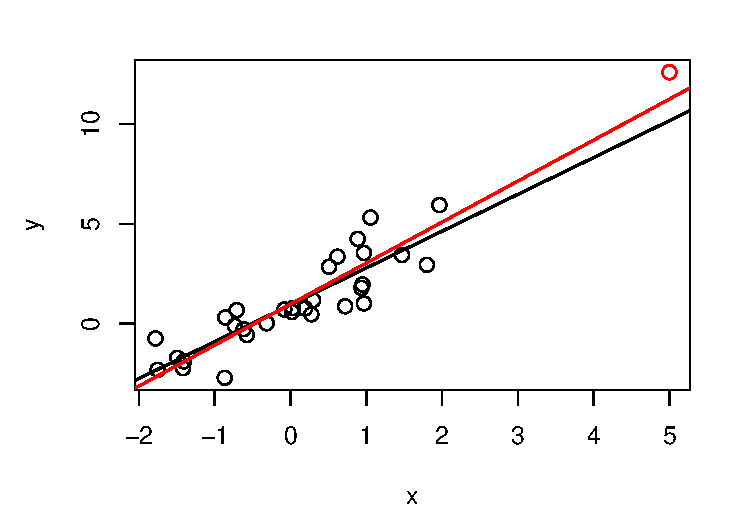
\includegraphics[scale=0.6]{figure/good_leverage.pdf}
\end{figure}
\end{center}

The red line is the least squares line including the high leverage point (red point).  The black line is the least squares line without the high leverage point.  
\end{frame}

%-----------------------------------------
\begin{frame}
Example of a ``bad" leverage point.  A ``bad" leverage point is a leverage point that is also an outlier.

\begin{center}
\begin{figure}
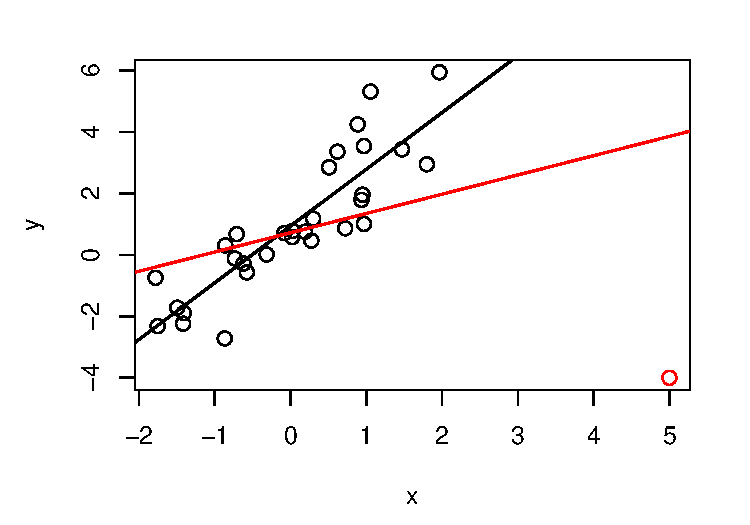
\includegraphics[scale=0.6]{figure/bad_leverage.pdf}
\end{figure}
\end{center}

The red line is the least squares line including the high leverage point (red point).  The black line is the least squares line without the high leverage point.  In this case, removing the high leverage point substantially changes the estimate of the least squares line. 
\end{frame}

%-----------------------------------------
\begin{frame}
Example of an outlier that is not a leverage point.

\begin{center}
\begin{figure}
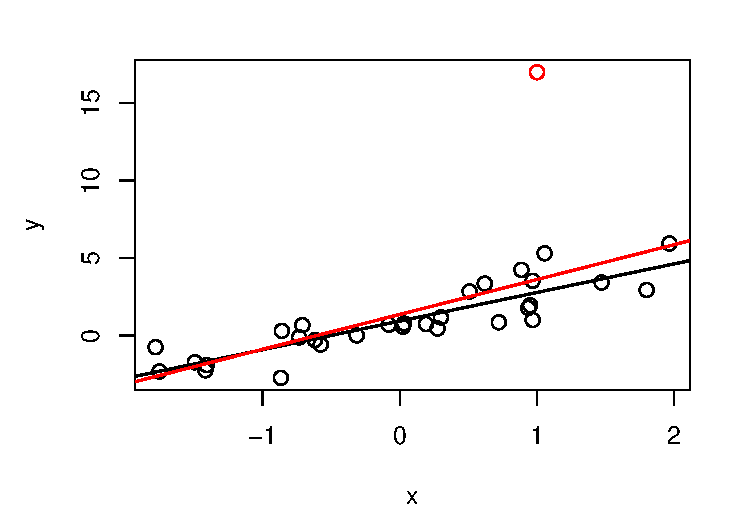
\includegraphics[scale=0.6]{figure/outlier.pdf}
\end{figure}
\end{center}

The red line is the least squares line including the outlier (red point).  The black line is the least squares line without the outlier.  
\end{frame}

%-----------------------------------------
\begin{frame}{Quantifying Leverage}
The \textbf{leverage} of the $i^{th}$ data point is quantified as
$$h_i = \frac{1}{n} + \frac{(x_i - \bar{x})^2}{\sum_{j=1}^n (x_j - \bar{x})^2}$$

\begin{itemize}
\item $h_i$ increases the further $x_i$ is from $\bar{x}$
\item $h_i$ is between $1/n$ and 1
\item For simple linear regression, average$(h_i) = 2/n$\\
\end{itemize}
\vspace{15pt}
\emph{See Sheather, Section 3.2.1, pp. 55-56 for a derivation}.
\end{frame}

%-----------------------------------------
\begin{frame}{Identifying Leverage Points}
A popular rule is to classify $x_i$ as a point of high leverage in a simple linear regression model if
$$h_i > 2 \times \text{average}(h_i) = 2 \times \frac{2}{n} = 4/n$$
\end{frame}


%-----------------------------------------
\begin{frame}{Residual Plots}
\begin{itemize}
\item One of the most useful diagnostics  is a plot of the residuals $\hat{e}_i = y_i - \hat{y}_i$ versus the fitted values $\hat{y}_i$, for $i=1, \cdots, n$.  It is also common to plot the reisduals $\hat{e}_i$ versus the predictor $x_i$.
\vspace{5pt}
\item One purpose of residual plots is to identify characteristics or patterns still apparent in the data after fitting the model.
\vspace{5pt}
\item Residual plots are especially useful for assessing linearity and constant variance.
\vspace{5pt}
\item Ideally, the residual plot should show no obvious pattern, and the points are randomly scattered around 0.
\end{itemize}
\end{frame}

%-----------------------------------------
\begin{frame}[fragile]{Residual Plots}
For the simple linear regression model of male weight versus height, the points in the residual plot look randomly scattered and show no obvious patterns, indicating that the assumptions are reasonably satisfied.  Although, there is one potential outlier.

\centering
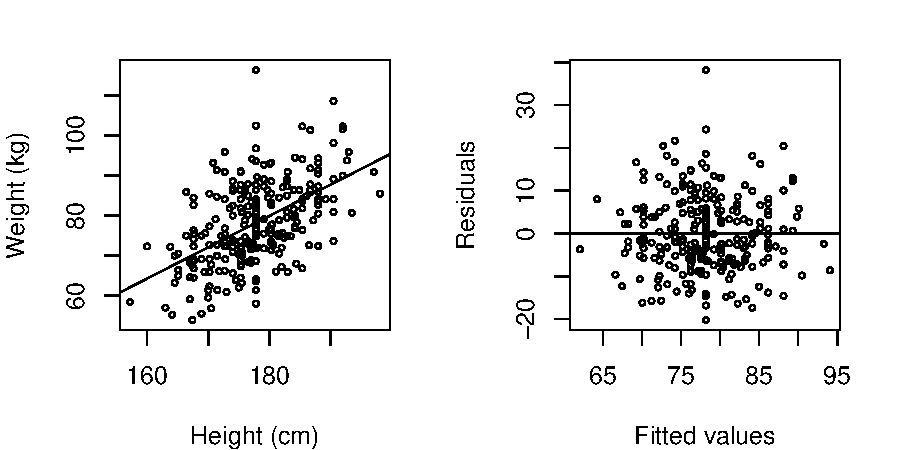
\includegraphics[scale=0.6]{figure/wgt_resid.pdf}
\end{frame}

%-----------------------------------------
\begin{frame}[fragile]
Here is the code used to create the last plot.
\small
\begin{verbatim}
> library(openintro)
> bdims_males <- subset(bdims, sex == 1) 
> lm1 <- lm(wgt ~ hgt, data=bdims_males)

> par(mfrow=c(1,2)) # split plot into 2 panes
# scatter plot with least squares line
> plot(wgt ~ hgt, data=bdims_males, 
       xlab = 'Height (cm)' , ylab = 'Weight (kg)')
> abline(lm1)

# residual plot
> plot(predict(lm1), resid(lm1), 
       xlab='Fitted values', ylab='Residuals')
> abline(h=0)
\end{verbatim}
\end{frame}

%-----------------------------------------
\begin{frame}{Residual Plots}
An example of nonconstant variance, also called \textbf{heteroscedasticity}.  The residual plot below shows a fan pattern.

\centering
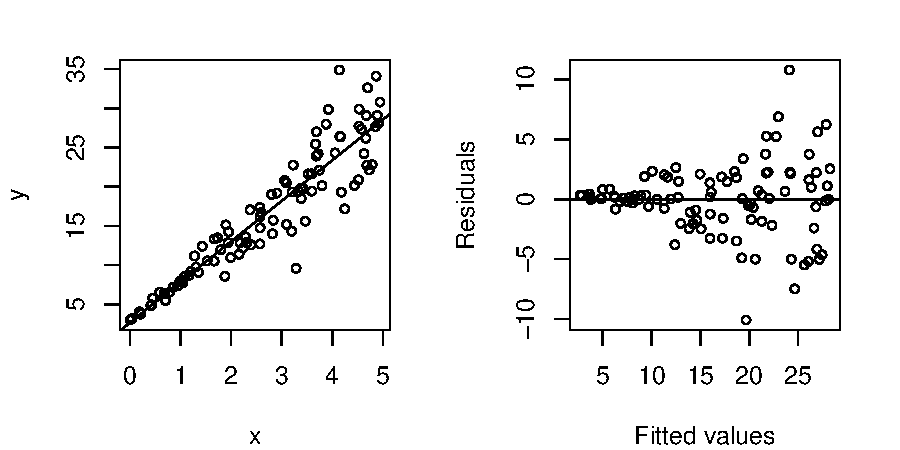
\includegraphics[scale=0.6]{figure/resid_var.pdf}
\end{frame}

%-----------------------------------------
\begin{frame}{Residual Plots}
An example of nonlinearity.

\centering
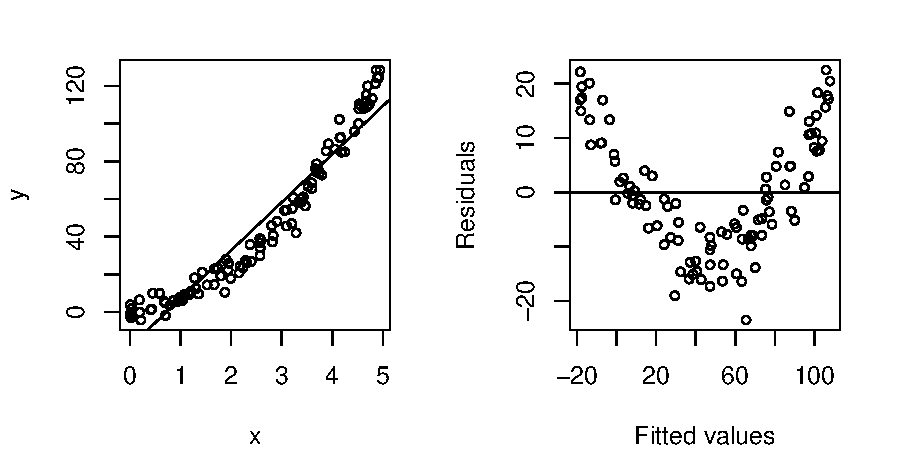
\includegraphics[scale=0.6]{figure/resid_nonlin.pdf}
\end{frame}

%-----------------------------------------
\begin{frame}{Question}
\vspace{-4cm}
\large
What is $\hat{e}_i$ and how is it different than $e_i$?
\end{frame}

%-----------------------------------------
\begin{frame}{Standardized Residuals}
It can be shown that the variance of the $i^{th}$ residual is given by
$$Var(\hat{e}_i) = \sigma^2 [1 - h_i],$$
where $h_i$ is the leverage of the $i^{th}$ point defined earlier. (See Sheather, Section 3.2.2, pp. 60-61, for a derivation.)\\
\vspace{15pt}

This implies residuals do not have equal variance, even though we make the assumption that the errors have constant variance $Var(e_i) = \sigma^2$.
\end{frame}

%-----------------------------------------
\begin{frame}{Standardized Residuals}
The problem of the residuals having different variances can be overcome by standardizing each residual by its standard error.  The $i^{th}$ standardized residual, $r_i$ is given by
$$r_i = \frac{\hat{e}_i}{\hat{\sigma} \sqrt{1 - h_{i}}},$$
where $\hat{\sigma} = \sqrt{\frac{1}{n-2} \sum_{i=1}^n \hat{e}_i^2}$ is the residual standard error (i.e., the estimate of $\sigma$)
\end{frame}

%-----------------------------------------
\begin{frame}{Standardized Residuals}
\begin{itemize}
\item A plot of the standardized residuals versus the fitted values is recommended when there are points of high leverage in a data set.\\
\vspace{10pt}
\item When there are no points of high leverage, there is generally little difference between the plot of the raw residuals and the standardized residuals.
\end{itemize}
\end{frame}

%-----------------------------------------
\begin{frame}{Identifying Outliers}
\begin{itemize}
\item One advantage of standardized residuals is that they inform us how many estimated standard errors any point is away from the fitted regression line. 
\begin{itemize}
\item For example, suppose that a point has a standardized residual of 4.3, then this point is 4.3 standard errors away from the fitted regression line, and would therefore be considered an outlier that should be investigated.\\
\end{itemize}
\vspace{5pt}
\item Sheather suggests labeling a point as an outlier if its standardized residual falls outside the interval from \textbf{-2 to 2}.  For large data sets, he suggests changing this rule to \textbf{-4 to 4} (otherwise, too many points would be flagged).
\end{itemize}
\end{frame}

%-----------------------------------------
\begin{frame}
To summarize the rules for identifying outliers and leverage points:
\vspace{5pt}
\begin{itemize}
\item An \textbf{outlier} is a point whose standardized residual falls outside the interval from \textbf{-2 to 2}
\vspace{5pt}
\item A \textbf{high leverage point} is a point that has $h_i > 4/n$ (note, this rule is only for simple linear regression)
\vspace{5pt}
\item A \textbf{``bad" leverage point} is leverage point that is also an outlier
\vspace{5pt}
\item A \textbf{``good" leverage point} is a leverage point that is not an outlier
\end{itemize}
\end{frame}

%-----------------------------------------
\begin{frame}[fragile]{Example: 2000 US Presidental Elections}
Data set with number of votes for George W. Bush and Pat Buchanan in Florida counties for the 2000 US presidential election.\\
\begin{verbatim}
> library(Stat2Data)
> data("PalmBeach")
> head(PalmBeach)
    County Buchanan   Bush
1  ALACHUA      262  34062
2    BAKER       73   5610
3      BAY      248  38637
4 BRADFORD       65   5413
5  BREVARD      570 115185
6  BROWARD      789 177279
\end{verbatim}
\end{frame}

%-----------------------------------------
\begin{frame}
\begin{itemize}
\item The 2000 presidential election between George W. Bush and Al Gore was very close, with the electoral college votes from Florida determining the outcome.
\vspace{10pt}
\item After a period of manual recounting, the Florida vote was ultimately settled in Bush's favor by a margin of 532 votes.\footnote{\url{https://en.wikipedia.org/wiki/2000_United_States_presidential_election_recount_in_Florida}}
\vspace{10pt}
\item About 2\% of the votes cast in Florida were awarded to other candidates, including the Reform Party candidate Pat Buchanan.
\end{itemize}
\end{frame}

%-----------------------------------------
\begin{frame}[fragile]
\begin{verbatim}
> lm1 <- lm(Buchanan ~ Bush, data=PalmBeach)
> plot(Buchanan ~ Bush, data=PalmBeach,
    ylab = "Buchanan votes", xlab = "Bush votes")
> abline(lm1)
\end{verbatim}
\begin{center}
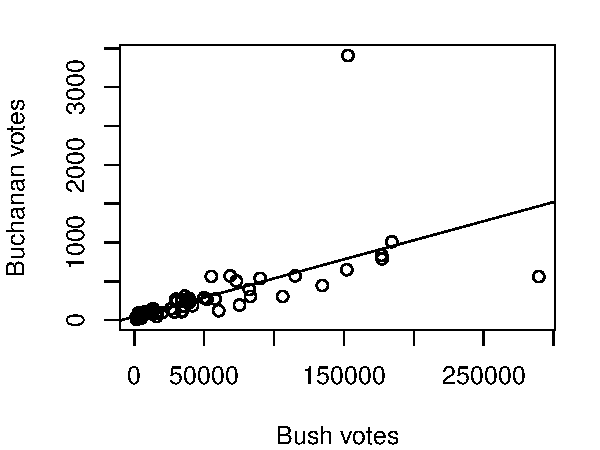
\includegraphics[scale=0.7]{figure/election_plot.pdf}
\end{center}
\end{frame}

%-----------------------------------------
\begin{frame}[fragile]
\begin{verbatim}
> plot(PalmBeach$Buchanan, rstandard(lm1),
    xlab = "Buchanan votes", ylab = "Standardized Residuals")
> abline(h=c(-2,2), lty=2)
\end{verbatim}
\begin{center}
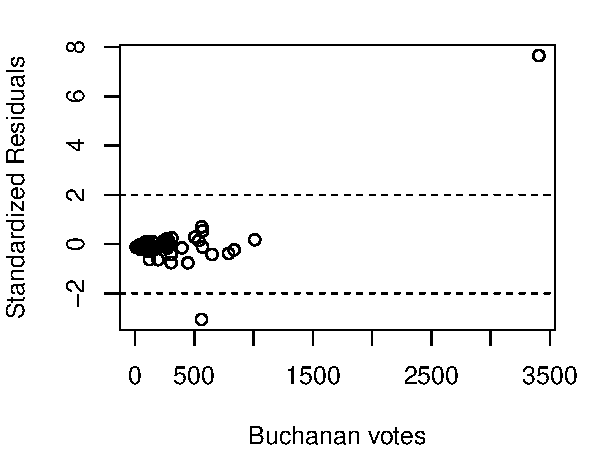
\includegraphics[scale=0.7]{figure/election_resid.pdf}
\end{center}
\end{frame}

%-----------------------------------------
\begin{frame}[fragile]
\begin{verbatim}
# identify outliers
> ind <- which(abs(rstandard(lm1)) > 2)
> PalmBeach[ind, ]
       County Buchanan   Bush
13       DADE      561 289456
50 PALM BEACH     3407 152846
\end{verbatim}
\end{frame}

%-----------------------------------------
\begin{frame}
\begin{itemize}
\item Palm Beach county used a unique ``butterfly ballot," which had a layout that was confusing for many voters.
\vspace{5pt}
\item Some voters that intedended to vote for Al Gore mistakenly marked their ballots for Pat Buchanan.  
\end{itemize}
\begin{center}
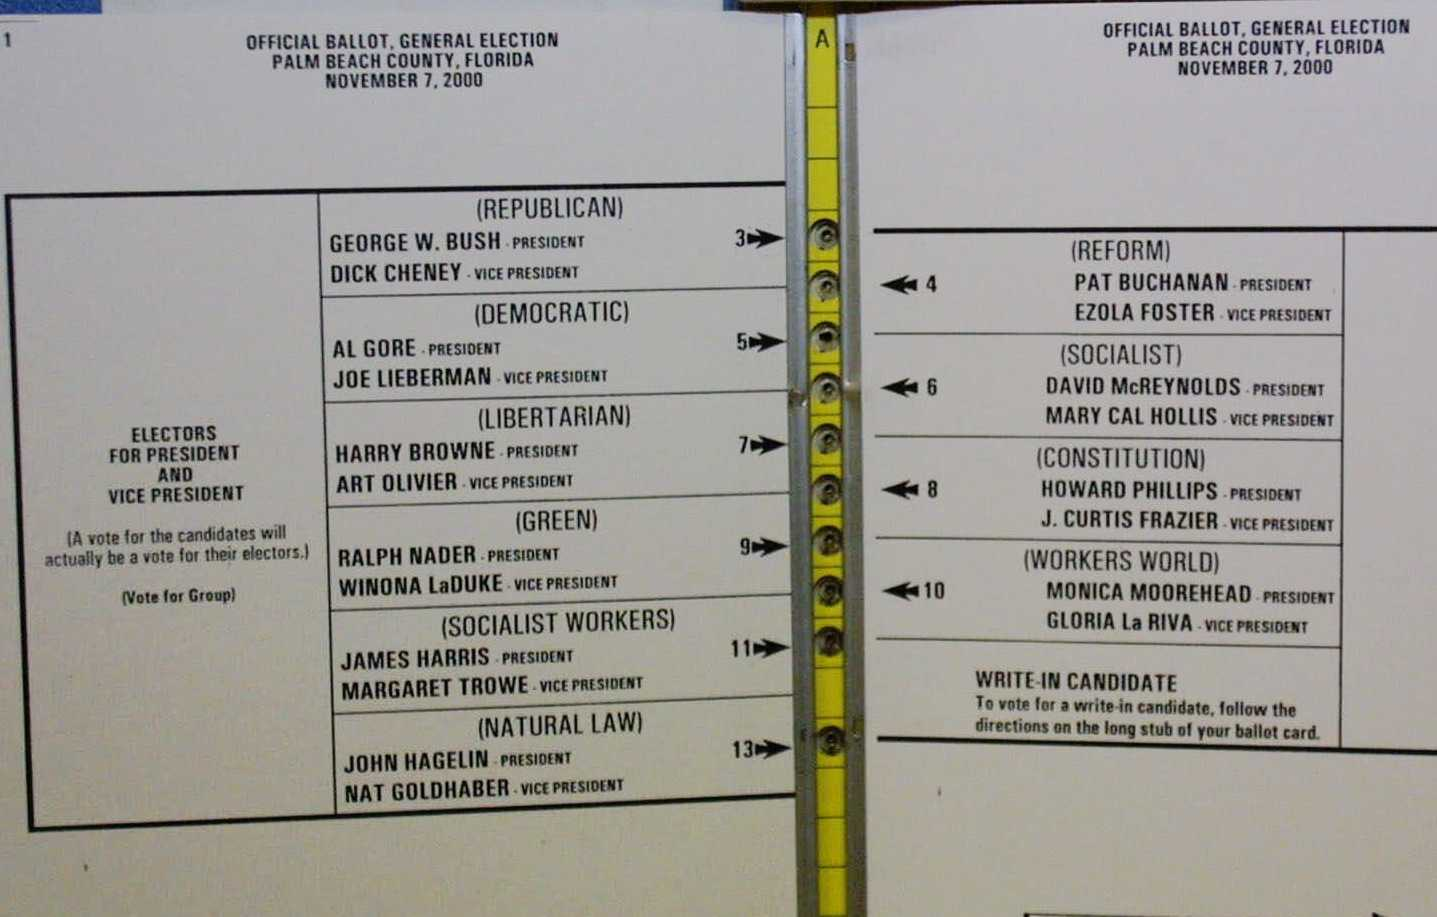
\includegraphics[scale=0.15]{figure/Butterfly_Ballot.jpg}
\end{center}
\tiny
Image Source:
\url{https://commons.wikimedia.org/wiki/File:Butterfly_Ballot,_Florida_2000_(large).jpg}

\end{frame}

%-----------------------------------------
\begin{frame}[fragile]
\begin{verbatim}
> plot(hatvalues(lm1), rstandard(lm1), 
    xlab = "Leverage", ylab = "Standardized Residuals")
> n <- nrow(PalmBeach)
> abline(v=4/n, lty=2) # threshold for high leverage
> abline(h=c(-2,2), lty=2) # threshold for outliers
\end{verbatim}
\begin{center}
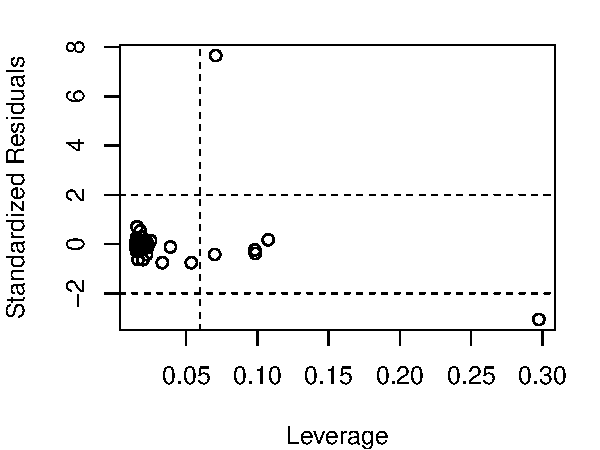
\includegraphics[scale=0.6]{figure/election_leverage.pdf}
\end{center}
\end{frame}

%-----------------------------------------
% \begin{frame}[fragile]
% \begin{verbatim}
% # identify bad leverage points
% > ind <- which(abs(rstandard(lm1)) > 2 & hatvalues(lm1) > 4/n)
% > PalmBeach[ind, ]
%        County Buchanan   Bush
% 13       DADE      561 289456
% 50 PALM BEACH     3407 152846
% \end{verbatim}
% \end{frame}

%-----------------------------------------
\begin{frame}{Question}
\vspace{-2cm}
Write R code that identifies those counties (rows) that correspond to high leverage points?\\
\vspace{3cm}

Write R code that identifies those counties that correspond to ``bad" leverage points?\\
\end{frame}
% also go over plot(lm1)



%-----------------------------------------
\begin{frame}
\textbf{Recommendations for handling outliers and leverage points:}
\vspace{5pt}
\begin{itemize}
\item Points should not be routinely deleted from an analysis because they do not fit the model.  Outliers and high leverage points should be carefully inspected.  There might be a data entry problem, or the points may be different than the rest of the data in some way (e.g., the ``butterfly ballots" in Palm Beach county).
\vspace{5pt}
\item Outliers and high leverage points may suggest an \textbf{alternative model}, in which the points are no longer unusual.  Consider including transformations, polynomial terms (e.g., $x$, $x^2$), or indicator variables.  These methods will be discussed in future lectures.
\end{itemize}
\end{frame}

% \begin{frame}
% \textbf{Remark}:  Some of the diagnostics considered here might seem excessive.  After all, for the election example, it was obvious, just by looking at the scatterplot that one county was unusual.\\  
% \vspace{10pt}
% 
% \textbf{However, all of these diagnostics will generalize to multiple regression modeling}.  For multiple regression modeling, we cannot simply inspect all our data on a two dimensional scatterplot, and so outliers and high leverage points are more difficult to detect without diagnostics.     
% \end{frame}

%-----------------------------------------
\begin{frame}{Assessing Normality (review)}
\begin{itemize}
\item A \textbf{normal probability plot}, or \textbf{normal QQ plot}, is a useful graphical technique for determining whether a data set follows an approximate normal distribution. 
\vspace{5pt}
\item Technically, a QQ plot is a plot of the sample quantiles (sorted data) on the $y$-axis, and the corresponding theoretical quantiles from the standard normal distribution on the $x$-axis.
\vspace{5pt}
\item If the points follow a straight line then the data are approximately normally distributed.  Any deviations form the straight line indicate deviations in the data from the normal distribution.
\vspace{5pt}
\item Histograms are also useful, but depend on arbitrary bin widths.  
\end{itemize}
\end{frame}

%-----------------------------------------
\begin{frame}[fragile]
For example, if we generate some data from a normal distribution using \texttt{rnorm()} then the points follow a straight line in the QQ plot.
\small
\begin{verbatim}
> set.seed(1)
> x <- rnorm(500)
> hist(x)
> qqnorm(x)
> qqline(x)
\end{verbatim}
\begin{center}
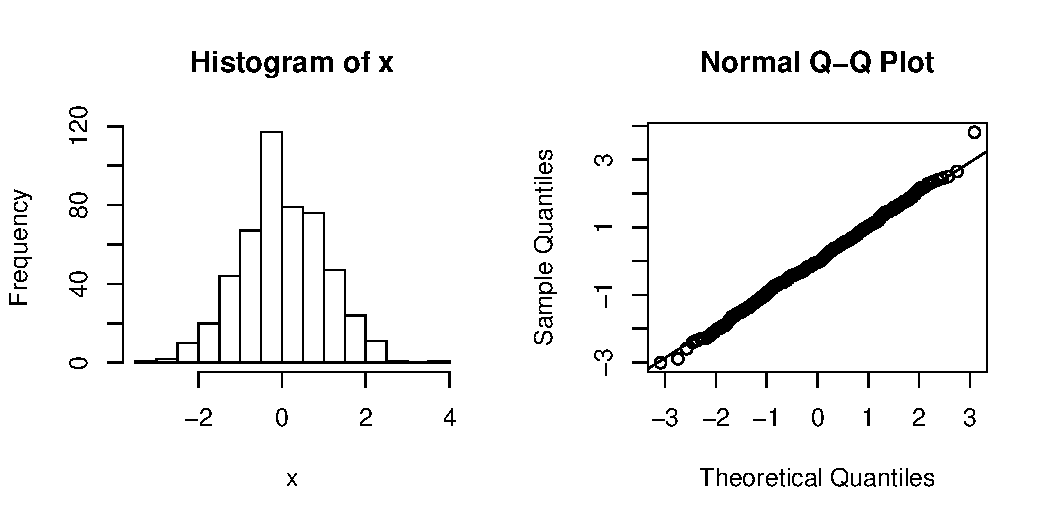
\includegraphics[scale=0.55]{figure/qqnorm1.pdf}
\end{center}
\end{frame}

%-----------------------------------------
\begin{frame}[fragile]
If the data do not follow a normal distribution, then there are deviations from the straight line.
\small
\begin{verbatim}
> set.seed(1)
> x <- rexp(500) # random numbers from an exponential distribution
> hist(x)
> qqnorm(x)
> qqline(x)
\end{verbatim}
\begin{center}
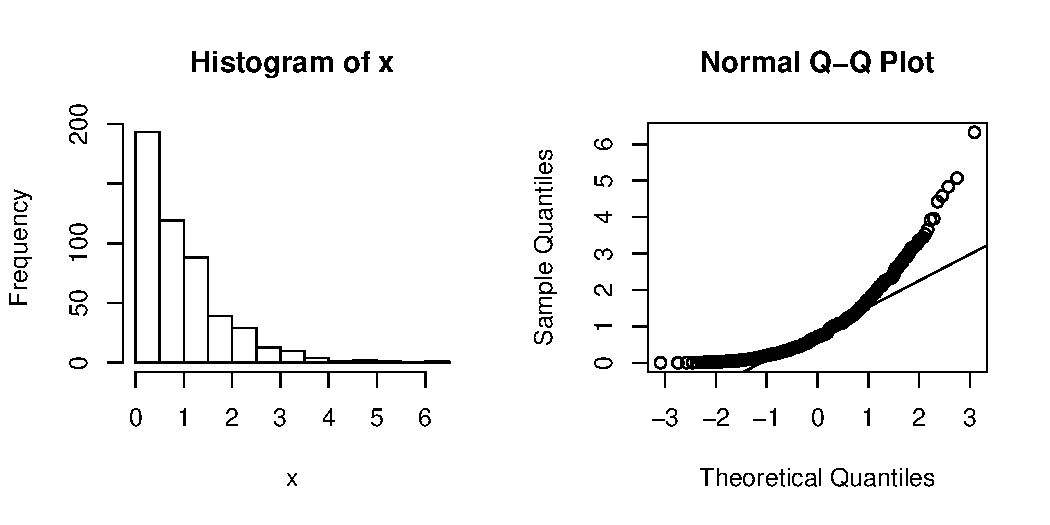
\includegraphics[scale=0.55]{figure/qqexp1.pdf}
\end{center}
\end{frame}

%-----------------------------------------
\begin{frame}[fragile]
It may not always be obvious from the histogram that the data are not normally distributed.
\small
\begin{verbatim}
> set.seed(1)
> x <- rt(500, df=5) # random numbers from an t-distribution
> hist(x)
> qqnorm(x)
> qqline(x)
\end{verbatim}
\begin{center}
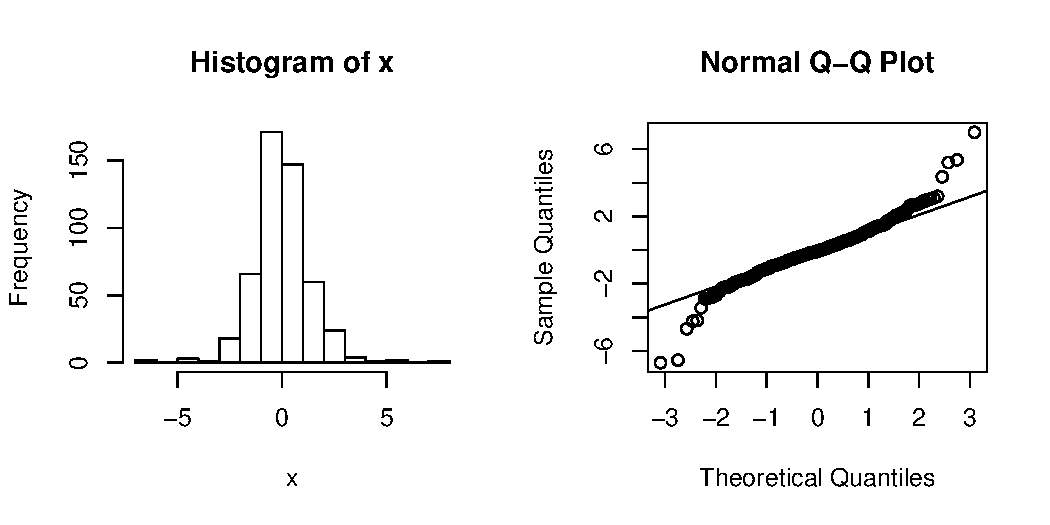
\includegraphics[scale=0.55]{figure/qqt1.pdf}
\end{center}
\end{frame}

%-----------------------------------------
\begin{frame}
\begin{itemize}
\item Recall that one of the assumptions for SLR is that the errors are normally distributed (i.e., $e_i \sim N(0, \sigma^2)$)
\vspace{10pt}
\item QQ plots and histograms are commonly used to check whether the residuals are normally distributed.  
\end{itemize}
\end{frame}

%-----------------------------------------
\begin{frame}[fragile]
For example, below is a QQ plot of the residuals for an SLR model of male weight versus height.  The points follow a straight line in the QQ plot, indicating that the residuals are approximately normal.  One observation is a potential outlier.
\small
\begin{verbatim}
> lm1 <- lm(wgt ~ hgt, data=bdims_males)
> hist(resid(lm1))
> qqnorm(resid(lm1))
> qqline(resid(lm1))
\end{verbatim}
\begin{center}
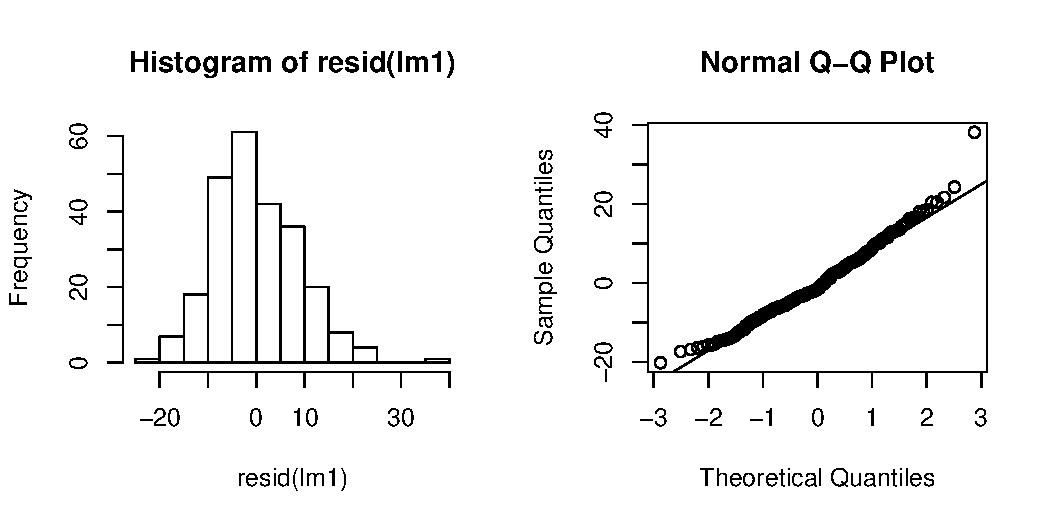
\includegraphics[scale=0.5]{figure/qqres.pdf}
\end{center}
\end{frame}

% \begin{frame}{}
% If you would like to read more about normal QQ-plots the following are good references:
% \vspace{5pt}
% \begin{itemize}
% \item OpenIntro Statistics, Ch.~3, Section 3.2, pp. 137--141.  Available here: \url{https://www.openintro.org/stat/textbook.php}
% \vspace{5pt}
% \item \url{https://www.itl.nist.gov/div898/handbook/eda/section3/normprpl.htm}
% \vspace{5pt}
% \item \url{https://en.wikipedia.org/wiki/Normal_probability_plot}\\
% \end{itemize}
% \end{frame}

% Assessing normality of residuals




\end{document}